\documentclass[a4paper]{book}
\usepackage[margin=1in]{geometry}
\usepackage[T1]{fontenc}
\usepackage[utf8]{inputenc}
\usepackage[hidelinks]{hyperref}
\usepackage{amsmath}
\usepackage{amssymb}
\usepackage{enumerate}
\usepackage{setspace}
\usepackage{listings}
\usepackage{xcolor}
\usepackage{amsthm}
\usepackage{xspace}
\usepackage{adjustbox}
\usepackage{booktabs} 
\usepackage{array}    
\usepackage{adjustbox} 
\usepackage{colortbl}
\usepackage{graphicx}


% Configuration pour les listings de code
\definecolor{codebg}{RGB}{245,245,245}
\lstset{
    backgroundcolor=\color{codebg},
    basicstyle=\ttfamily\small,
    frame=single,
    breaklines=true,
    columns=fullflexible,
    keywordstyle=\color{blue},
    commentstyle=\color{gray},
    stringstyle=\color{orange},
    showstringspaces=false
}
\setstretch{1.15}

%----- TITLE PAGE INFO -----%
\title{\Huge \textbf{Spanning Tree Protocol (STP) Workbook}\\
       \Large Fundamentals, Variants, Tuning, and Practical Labs}
\author{\Large Written for Networking Students and Professionals}
\date{\today}

\begin{document}

%----- MODERN TITLE PAGE -----%
\begin{titlepage}
    \centering

    \vspace*{4cm}
    {\Huge \textbf{VLAN Trunking Protocol (VTP) Workbook}\par}
    \vspace{0.8cm}
    {\Large A Hands-On Guide to Configuration, VLAN Management, and Troubleshooting\par}
    \vspace{0.3cm}
    \rule{0.9\textwidth}{1pt}
    
    \vspace{0.6cm}
    {\large \textbf{Mehdi JAFARI ZADEH}}\par
    \vspace{0.3cm}

    
    \vfill
    \textbf{Date:} \today
    \vspace{2cm}
\end{titlepage}


\tableofcontents

\chapter{VTP (VLAN Trunking Protocol) Tutorial}

\section{Introduction to VTP}
\subsection{What is VTP?}
VTP (VLAN Trunking Protocol) is a Cisco proprietary protocol that manages VLAN configurations across multiple switches in a network. It allows for:
\begin{itemize}
    \item \textbf{Centralized VLAN Management} – VLANs created on one switch (VTP Server) propagate to other switches (VTP Clients).
    \item \textbf{Consistency} – Ensures VLAN information remains synchronized across switches.
    \item \textbf{Reduced Configuration Errors} – Prevents VLAN mismatches.
    \item \textbf{Efficient VLAN Management} – Reduces administrative overhead.
\end{itemize}

\subsection{Network Topology Overview}
This tutorial follows the given network topology:

\begin{figure}[h]
    \centering
    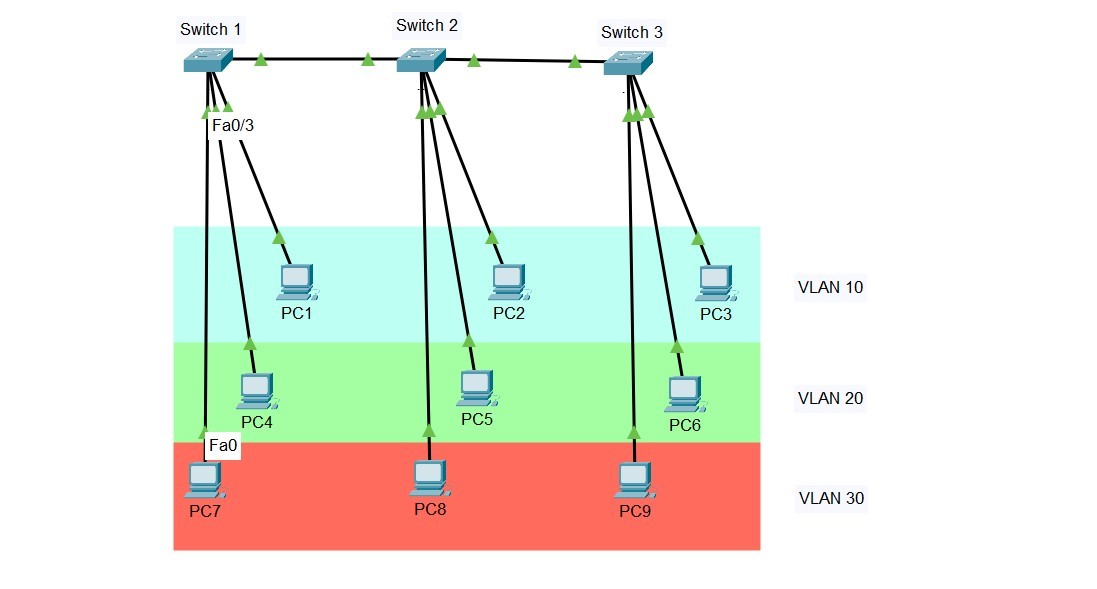
\includegraphics[width=0.9\textwidth]{network_topology.jpg}
    \caption{\textit{Network topology created using the Packet Tracer Simulator.}}

    \label{fig:packet_tracer_topology}
\end{figure}


\begin{itemize}
    \item \textbf{Three Switches}: Switch 1, Switch 2, Switch 3
    \item \textbf{Nine PCs connected to VLANs}:
    \begin{itemize}
        \item VLAN 10: PC1 (Switch 1), PC2 (Switch 2), PC3 (Switch 3)
        \item VLAN 20: PC4 (Switch 1), PC5 (Switch 2), PC6 (Switch 3)
        \item VLAN 30: PC7 (Switch 1), PC8 (Switch 2), PC9 (Switch 3)
    \end{itemize}
    \item \textbf{Switch Connections}: 
    \begin{itemize}
        \item Switch 1 connected to Switch 2
        \item Switch 2 connected to Switch 3
    \end{itemize}
\end{itemize}

\section{VTP Modes}
Cisco switches support three VTP modes:

\begin{table}[h]
    \centering
    \begin{tabular}{|c|p{10cm}|}
        \hline
        \textbf{Mode} & \textbf{Description} \\
        \hline
        Server & Creates, modifies, and deletes VLANs. Sends VTP updates. \\
        \hline
        Client & Receives and synchronizes VLANs from the VTP server. Cannot create VLANs. \\
        \hline
        Transparent & Does not participate in VTP updates but forwards them. Can create local VLANs. \\
        \hline
    \end{tabular}
    \caption{VTP Modes in Cisco Switches}
\end{table}

For our topology:
\begin{itemize}
    \item \textbf{Switch 1 is the VTP Server}.
    \item \textbf{Switch 2 and Switch 3 are VTP Clients}.
\end{itemize}

\section{Configuring VTP}
\subsection{Step 1: Configure VTP on Switch 1 (Server Mode)}
Set the VTP domain name, enable server mode, set a password, and enable version 2.
\begin{lstlisting}
Switch1(config)# vtp domain NetworkingLab
Switch1(config)# vtp mode server
Switch1(config)# vtp password cisco123
Switch1(config)# vtp version 2
\end{lstlisting}

\subsection{Step 2: Configure VTP on Switch 2 and Switch 3 (Client Mode)}
\begin{lstlisting}
Switch2(config)# vtp domain NetworkingLab
Switch2(config)# vtp mode client
Switch2(config)# vtp password cisco123
Switch2(config)# vtp version 2

Switch3(config)# vtp domain NetworkingLab
Switch3(config)# vtp mode client
Switch3(config)# vtp password cisco123
Switch3(config)# vtp version 2
\end{lstlisting}

\subsection{Step 3: Verify VTP Configuration}
\begin{lstlisting}
Switch1# show vtp status
Switch2# show vtp status
Switch3# show vtp status
\end{lstlisting}

\section{VTP VLAN Management}
\subsection{Step 4: Create VLANs on Switch 1 (VTP Server Mode)}
\begin{lstlisting}
Switch1(config)# vlan 10
Switch1(config-vlan)# name VLAN10
Switch1(config)# vlan 20
Switch1(config-vlan)# name VLAN20
Switch1(config)# vlan 30
Switch1(config-vlan)# name VLAN30
\end{lstlisting}

\subsection{Step 5: Verify VLAN Propagation}
\begin{lstlisting}
Switch2# show vlan brief
Switch3# show vlan brief
\end{lstlisting}

\section{Assigning VLANs to Interfaces}
\subsection{Step 6: Assign VLANs to PCs}
\begin{lstlisting}
Switch1(config)# interface fa0/3
Switch1(config-if)# switchport mode access
Switch1(config-if)# switchport access vlan 10

Switch2(config)# interface fa0/3
Switch2(config-if)# switchport mode access
Switch2(config-if)# switchport access vlan 10

Switch3(config)# interface fa0/3
Switch3(config-if)# switchport mode access
Switch3(config-if)# switchport access vlan 10
\end{lstlisting}

\section{VTP Troubleshooting}
\subsection{Checking and Resetting VTP}
\begin{lstlisting}
Switch1# show vtp status
Switch3# vtp mode transparent
Switch3# vtp mode client
Switch2(config)# debug sw-vlan vtp events
\end{lstlisting}

\section{VTP Pruning}
\subsection{Enabling VTP Pruning}
\begin{lstlisting}
Switch1(config)# vtp pruning
\end{lstlisting}
Verify pruning:
\begin{lstlisting}
Switch1# show vtp status
\end{lstlisting}

\section{Summary}
\begin{itemize}
    \item VTP allows automatic VLAN propagation in a network.
    \item Switch 1 (VTP Server) manages VLANs, while Switch 2 and 3 (Clients) receive updates.
    \item VLANs should be created on the VTP Server.
    \item Use trunk links between switches for VLAN traffic.
    \item VTP Pruning helps optimize VLAN traffic.
\end{itemize}

\chapter{Exercises (Practice Section)}
\section{Basic VTP Configuration Exercises}

\begin{enumerate}
    \item Configure \textbf{Switch 1} as the \textbf{VTP server} for the domain \texttt{"NetworkingLab"} with password \texttt{"cisco123"}.
    \item Configure \textbf{Switch 2} and \textbf{Switch 3} as \textbf{VTP clients} in the \texttt{"NetworkingLab"} domain with password \texttt{"cisco123"}.
    \item Change \textbf{Switch 3} to \textbf{VTP transparent mode} while keeping it in the \texttt{"NetworkingLab"} domain.
    \item Set \textbf{VTP version 2} on all switches.
    \item Configure \textbf{Switch 2} with a \textbf{VTP pruning feature enabled}.
    \item Reset the \textbf{VTP configuration} on \textbf{Switch 1} to default.
    \item Change the \textbf{VTP domain name} from \texttt{"NetworkingLab"} to \texttt{"CiscoNet"} on \textbf{Switch 1}.
    \item Verify the \textbf{VTP configuration} on \textbf{Switch 3}.
    \item Disable \textbf{VTP pruning} on \textbf{Switch 2}.
    \item Check the \textbf{VTP mode} of \textbf{Switch 3}.
\end{enumerate}

\newpage

\section{VTP and VLAN Management Exercises}

\begin{enumerate}
    \item Create VLAN 10, VLAN 20, and VLAN 30 on \textbf{Switch 1} in \textbf{VTP Server mode}.
    \item Assign \textbf{PC1, PC2, and PC3} to \textbf{VLAN 10} on their respective switches.
    \item Assign \textbf{PC4, PC5, and PC6} to \textbf{VLAN 20} on their respective switches.
    \item Assign \textbf{PC7, PC8, and PC9} to \textbf{VLAN 30} on their respective switches.
    \item Verify if \textbf{VLAN 10, VLAN 20, and VLAN 30} are properly propagated to \textbf{Switch 2} and \textbf{Switch 3}.
    \item Remove \textbf{VLAN 30} from \textbf{Switch 1} and observe if the deletion propagates to other switches.
    \item Add a new \textbf{VLAN 40} to \textbf{Switch 1} and check if it appears in \textbf{Switch 2 and Switch 3}.
    \item Change the name of \textbf{VLAN 20} to \texttt{"StudentNetwork"} on \textbf{Switch 1} and verify if it propagates.
    \item Delete \textbf{VLAN 10} on \textbf{Switch 1} and check if it is removed from \textbf{Switch 2 and Switch 3}.
    \item On \textbf{Switch 2}, verify if \textbf{VTP pruning} is active.
\end{enumerate}
\newpage

\section{Troubleshooting and Debugging VTP Exercises}


\begin{enumerate}
    \item The VLANs are not propagating to \textbf{Switch 3}. Verify the \textbf{VTP domain name}.
    \item \textbf{Switch 3} is in \textbf{transparent mode}, but VLANs are not being updated. Change it to \textbf{client mode}.
    \item Verify the \textbf{VTP revision number} on \textbf{Switch 2}.
    \item Check the \textbf{VTP configuration revision number} mismatch issue on \textbf{Switch 1}.
    \item Show the \textbf{VTP password} on \textbf{Switch 3}.
    \item The \textbf{VLAN database is not updating} on \textbf{Switch 2}. Check and reset the VTP configuration.
    \item Debug and display \textbf{VTP updates} on \textbf{Switch 1}.
    \item Restore the default \textbf{VTP mode} on \textbf{Switch 3}.
    \item Force \textbf{Switch 1} to send \textbf{VTP updates} manually.
    \item Change \textbf{Switch 2} to \textbf{VTP off mode} to prevent VLAN propagation.
\end{enumerate}
\newpage

\chapter{Answer Key (Solutions Section)}
\section{Basic VTP Configuration Answers}

\begin{enumerate}
    \item \textbf{Configure Switch 1 as the VTP server:}
    \begin{lstlisting}
    Switch1(config)# vtp domain NetworkingLab
    Switch1(config)# vtp mode server
    Switch1(config)# vtp password cisco123
    \end{lstlisting}

    \item \textbf{Configure Switch 2 and Switch 3 as VTP clients:}
    \begin{lstlisting}
    Switch2(config)# vtp domain NetworkingLab
    Switch2(config)# vtp mode client
    Switch2(config)# vtp password cisco123

    Switch3(config)# vtp domain NetworkingLab
    Switch3(config)# vtp mode client
    Switch3(config)# vtp password cisco123
    \end{lstlisting}

    \item \textbf{Change Switch 3 to VTP Transparent mode:}
    \begin{lstlisting}
    Switch3(config)# vtp mode transparent
    \end{lstlisting}

    \item \textbf{Set VTP version 2 on all switches:}
    \begin{lstlisting}
    Switch1(config)# vtp version 2
    Switch2(config)# vtp version 2
    Switch3(config)# vtp version 2
    \end{lstlisting}

    \item \textbf{Enable VTP pruning on Switch 2:}
    \begin{lstlisting}
    Switch2(config)# vtp pruning
    \end{lstlisting}

    \item \textbf{Reset VTP configuration on Switch 1:}
    \begin{lstlisting}
    Switch1(config)# vtp mode transparent
    Switch1(config)# vtp mode server
    \end{lstlisting}

    \item \textbf{Change the VTP domain name from "NetworkingLab" to "CiscoNet" on Switch 1:}
    \begin{lstlisting}
    Switch1(config)# vtp domain CiscoNet
    \end{lstlisting}

    \item \textbf{Verify VTP configuration on Switch 3:}
    \begin{lstlisting}
    Switch3# show vtp status
    \end{lstlisting}

    \item \textbf{Disable VTP pruning on Switch 2:}
    \begin{lstlisting}
    Switch2(config)# no vtp pruning
    \end{lstlisting}

    \item \textbf{Check VTP mode of Switch 3:}
    \begin{lstlisting}
    Switch3# show vtp status
    \end{lstlisting}
\end{enumerate}

\section{VTP and VLAN Management Answers}

\begin{enumerate}
    \item \textbf{Create VLAN 10, VLAN 20, and VLAN 30 on Switch 1 (VTP Server Mode):}
    \begin{lstlisting}
    Switch1(config)# vlan 10
    Switch1(config-vlan)# name VLAN10
    Switch1(config)# vlan 20
    Switch1(config-vlan)# name VLAN20
    Switch1(config)# vlan 30
    Switch1(config-vlan)# name VLAN30
    \end{lstlisting}

    \item \textbf{Assign PC1, PC2, and PC3 to VLAN 10 on their respective switches:}
    \begin{lstlisting}
    Switch1(config)# interface fa0/3
    Switch1(config-if)# switchport mode access
    Switch1(config-if)# switchport access vlan 10

    Switch2(config)# interface fa0/3
    Switch2(config-if)# switchport mode access
    Switch2(config-if)# switchport access vlan 10

    Switch3(config)# interface fa0/3
    Switch3(config-if)# switchport mode access
    Switch3(config-if)# switchport access vlan 10
    \end{lstlisting}

    \item \textbf{Assign PC4, PC5, and PC6 to VLAN 20 on their respective switches:}
    \begin{lstlisting}
    Switch1(config)# interface fa0/4
    Switch1(config-if)# switchport mode access
    Switch1(config-if)# switchport access vlan 20

    Switch2(config)# interface fa0/4
    Switch2(config-if)# switchport mode access
    Switch2(config-if)# switchport access vlan 20

    Switch3(config)# interface fa0/4
    Switch3(config-if)# switchport mode access
    Switch3(config-if)# switchport access vlan 20
    \end{lstlisting}

    \item \textbf{Assign PC7, PC8, and PC9 to VLAN 30 on their respective switches:}
    \begin{lstlisting}
    Switch1(config)# interface fa0/5
    Switch1(config-if)# switchport mode access
    Switch1(config-if)# switchport access vlan 30

    Switch2(config)# interface fa0/5
    Switch2(config-if)# switchport mode access
    Switch2(config-if)# switchport access vlan 30

    Switch3(config)# interface fa0/5
    Switch3(config-if)# switchport mode access
    Switch3(config-if)# switchport access vlan 30
    \end{lstlisting}

    \item \textbf{Verify if VLAN 10, 20, and 30 are properly propagated to Switch 2 and Switch 3:}
    \begin{lstlisting}
    Switch2# show vlan brief
    Switch3# show vlan brief
    \end{lstlisting}

    \item \textbf{Remove VLAN 30 from Switch 1 and verify propagation:}
    \begin{lstlisting}
    Switch1(config)# no vlan 30
    \end{lstlisting}

    \item \textbf{Add VLAN 40 to Switch 1 and verify propagation:}
    \begin{lstlisting}
    Switch1(config)# vlan 40
    Switch1(config-vlan)# name VLAN40
    \end{lstlisting}

    \item \textbf{Change the name of VLAN 20 to "StudentNetwork" on Switch 1 and verify propagation:}
    \begin{lstlisting}
    Switch1(config)# vlan 20
    Switch1(config-vlan)# name StudentNetwork
    \end{lstlisting}

    \item \textbf{Delete VLAN 10 from Switch 1 and check if it is removed from Switch 2 and Switch 3:}
    \begin{lstlisting}
    Switch1(config)# no vlan 10
    \end{lstlisting}

    \item \textbf{On Switch 2, verify if VTP pruning is active:}
    \begin{lstlisting}
    Switch2# show vtp status
    \end{lstlisting}
\end{enumerate}

\section{Troubleshooting and Debugging VTP Answers}

\begin{enumerate}
    \item \textbf{The VLANs are not propagating to Switch 3. Verify the VTP domain name:}
    \begin{lstlisting}
    Switch3# show vtp status
    \end{lstlisting}

    \item \textbf{Switch 3 is in transparent mode, but VLANs are not being updated. Change it to client mode:}
    \begin{lstlisting}
    Switch3(config)# vtp mode client
    \end{lstlisting}

    \item \textbf{Verify the VTP revision number on Switch 2:}
    \begin{lstlisting}
    Switch2# show vtp status
    \end{lstlisting}

    \item \textbf{Check for VTP configuration revision number mismatch on Switch 1:}
    \begin{lstlisting}
    Switch1# show vtp status
    \end{lstlisting}

    \item \textbf{Show the VTP password on Switch 3:}
    \begin{lstlisting}
    Switch3# show vtp password
    \end{lstlisting}

    \item \textbf{The VLAN database is not updating on Switch 2. Check and reset the VTP configuration:}
    \begin{lstlisting}
    Switch2(config)# vtp mode transparent
    Switch2(config)# vtp mode client
    \end{lstlisting}

    \item \textbf{Debug and display VTP updates on Switch 1:}
    \begin{lstlisting}
    Switch1# debug sw-vlan vtp events
    \end{lstlisting}

    \item \textbf{Restore the default VTP mode on Switch 3:}
    \begin{lstlisting}
    Switch3(config)# vtp mode server
    \end{lstlisting}

    \item \textbf{Force Switch 1 to send VTP updates manually:}
    \begin{lstlisting}
    Switch1(config)# vtp mode transparent
    Switch1(config)# vtp mode server
    \end{lstlisting}

    \item \textbf{Change Switch 2 to VTP off mode to prevent VLAN propagation:}
    \begin{lstlisting}
    Switch2(config)# vtp mode off
    \end{lstlisting}
\end{enumerate}

\end{document}
